\documentclass{beamer}

\usetheme[secheader]{Boadilla}
\usecolortheme{crane}
\usepackage[latin1]{inputenc}

\title{Open Source Android Development Tools}
\author{Manfred Moser}
\date{June, 2011}
\institute[2011]{simpligility technologies inc.}

\begin{document}

\begin{frame}
  \titlepage 
\end{frame}

\begin{frame}
  \frametitle{Table of Contents}
  SDK, ADT and beyond
  \setcounter{tocdepth}{1}
  \tableofcontents
\end{frame}


\section{Android Itself}

  \subsection{Components}
    \begin{frame}
      \frametitle{What Components make up Android?}
      \begin{itemize}
        \item<1->Android Proper
        \item<2->AOSP
        \item<3->ADT
      \end{itemize}
    \end{frame}

  \subsection{Android Proper}
    \begin{frame}
    \frametitle{Android Proper}
    \begin{itemize}
      \item<1->Linux
      \item Apache Harmony 
      \item<2->Lots of other open source components
      \item<3->AOSP bits
      \item<4->binary device driver and other blobs
    \end{itemize}
    \end{frame}
  
  \subsection{AOSP}
    \begin{frame}
      \frametitle{Android Open Source Project AOSP}
      \begin{itemize}
        \item<1->open source drops
        \item<2->base for custom roms and such
        \item<3->ADT
      \end{itemize}
    \end{frame}

  \subsection{ADT}
    \begin{frame}
      \frametitle{Android Development Toolkit ADT}
      \begin{itemize}
        \item<1->open source, fully 
        \item<2->EPL
      \end{itemize}
    \end{frame}

\section{Development Tools}

  \subsection{IDEs}

    \begin{frame}
      \frametitle{Eclipse and ADT and friends}
    \end{frame}

    \begin{frame}
      \frametitle{Motorola Motodev Studio for Android}
    \end{frame}

    \begin{frame}
      \frametitle{Jetbrains IntelliJ IDEA CE}
    \end{frame}

    \begin{frame}
      \frametitle{Oracle Netbeans}
    \end{frame}

    \begin{frame}
      \frametitle{Others}
        \begin{itemize}
        \item<1->DroidDraw
        \item<2->EPL
      \end{itemize}
    \end{frame}

\subsection{Build Tools}

\begin{frame}
  \frametitle{Ant}
\end{frame}

\begin{frame}
  \frametitle{Maven Android Plugin}
\end{frame}

\begin{frame}
  \frametitle{Gradle Android Plugin}
\end{frame}

\begin{frame}
  \frametitle{SBT Android Plugin}
\end{frame}

\subsection{Other Languages}
\begin{frame}
  \frametitle{JRuby}
\end{frame}

\begin{frame}
  \frametitle{Scala}
\end{frame}

\begin{frame}
  \frametitle{Csharp}
\end{frame}

\subsection{Other Development Tools}

\begin{frame}
  \frametitle{Other Development Tools}
  \begin{itemize}
    \item<1->Droid at Screen 
    \item<2->dex2jar and others
  \end{itemize}
\end{frame}

\section{Development Libraries}
\subsection{Java Libraries}

\begin{frame}
  \frametitle{}
  \begin{itemize}
    \item<1->jackson
    \item<2->dex2jar and others
  \end{itemize}
\end{frame}

\subsection{Android Specific Libraries}

\begin{frame}
  \frametitle{Android Specific Libraries}
  \begin{itemize}
    \item<1->Roboguice 
    \item<2->Androidannotations
    \item<3->DroidFu
    \item<4->GreenDroid
    \item<5->AndEngine
    \item<6->http://actionbarsherlock.com/
  \end{itemize}
\end{frame}

\subsection{Android UI Libraries}

\begin{frame}
  \frametitle{AndroidSherlock}
  \begin{center}
  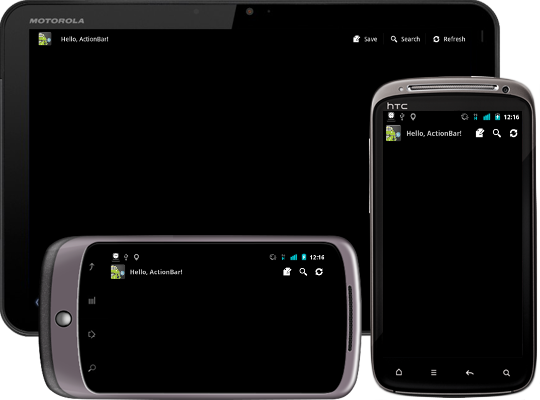
\includegraphics[height=1.0in]{androidsherlock.png}
  \end{center}
\end{frame}

\subsection{Android Testing Libraries}

\begin{frame}
  \frametitle{Android Testing Libraries}
  \begin{itemize}
    \item<1->Robotium 
    \item<2->Robolectric
    \item<3->Calculon
    \item<4->unit test copy tool
  \end{itemize}
\end{frame}


\subsection{Others of interest} 

\begin{frame}
  \frametitle{i-jetty}
\end{frame}

\begin{frame}
  \frametitle{web based frameworks}
\end{frame}

\subsection{Conclusions}

\begin{frame}
  \frametitle{Is Android Java}
  no, not only, yes .. a hell of a lot is,
  combination of things, pull communities together
\end{frame}

\begin{frame}
  \frame{Is Android Open Source}

yes and no, both, lots of it is, stronger community can push to more openness

\end{frame}

\begin{frame}
 \frame {Overall conclusion}

Despite a lot of flaws and things
Android rocks and is Open Source and Java and a whole lot more
\end{frame}


\end{document}